\documentclass{article}
\usepackage[utf8]{inputenc}
\usepackage{lipsum}
\usepackage{graphicx} 
\graphicspath{ {./images/} }
\title{2022ss-inftech: LATEX exercise}
\author{Sankalp Chordia}
\date{January 2023}

\begin{document}

\maketitle


\section{Special relativity}

\hrule
\vspace{5pt}


Special relativity is a theory of the structure of spacetime. It was introduced in Einstein's 1905 paper "On the Electrodynamics of Moving Bodies" (for the contributions of many other physicists and mathematicians, see History of special relativity). Special relativity is based on two postulates which are contradictory in classical mechanics:
\vspace{5pt}

1.The laws of physics are the same for all observers in any inertial frame of reference relative to one another (principle of relativity).
\vspace{3pt}

2.The speed of light in a vacuum is the same for all observers, regardless of their relative motion or of the motion of the light source.
\vspace{10pt}

The resultant theory copes with experiment better than classical mechanics. For instance, postulate 2 explains the results of the Michelson–Morley experiment. Moreover, the theory has many surprising and counterintuitive consequences. Some of these are:



   \begin{itemize}
     \item Relativity of simultaneity: Two events, simultaneous for one observer, may not be simultaneous for another observer if the observers are in relative motion.
     \item Time dilation: Moving clocks are measured to tick more slowly than an observer's "stationary" clock.
     \item Length contraction: Objects are measured to be shortened in the direction that they are moving with respect to the observer.
     \item Maximum speed is finite: No physical object, message or field line can travel faster than the speed of light in a vacuum.
      \begin{itemize}
      \item [•]The effect of gravity can only travel hrough space at the speed of light, not faster or instantaneously.
      \end{itemize}
    \item Mass–energy equivalence: E = mc2, energy and mass are equivalent and transmutable.
    \item Relativistic mass, idea used by some researchers.
    \end{itemize}
    The defining feature of special relativity is the replacement of the Galilean transformations of classical mechanics by the Lorentz transformations. (See Maxwell's equations of electromagnetism.)
    
     
     
\vspace{5pt}

\vspace{15pt}
\begin{center}
 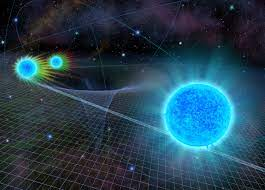
\includegraphics{images/image1.jpeg}   
\end{center}


\pagebreak

\section{Mass–velocity relationship}
\hrule
\vspace{25pt}
\begin{center}
    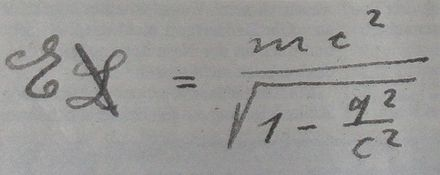
\includegraphics{images/image2.jpeg}
\end{center}
In developing special relativity, Einstein found that the kinetic energy of a moving body is
\vspace{10pt}
\begin{equation}
    E_k=m_0c^2(\gamma - 1 ) = m_0c^2(1/(\sqrt{1-v^2/c^2}-1) ,
    \end{equation}
    
    with v the velocity, m_0$ the rest mass, and \gamma$ the  Lorentz factor.

\vspace{10pt}

He included the second term on the right to make sure that for small velocities the energy would be the same as in classical mechanics, thus satisfying the correspondence principle:
\begin{equation}
    \vspace{10pt}
    E_k=1/2(m_0v^2)+.....    
\end{equation}
Without this second term, there would be an additional contribution in the energy when the particle is not moving.

\end{document}
